Docker ofrece un mecanismo de comunicación con un entorno aislado llamado contenedor,
que ha sido introducido anteriormente. Los contenedores por defecto están aislados,
son seguros y empaquetan todo lo necesario para funcionar, por lo que no necesitan
nada del sistema que está por debajo.

Internamente, Docker utiliza la arquitectura ``cliente--servidor'' para gestionar tanto
las comunicaciones y contenedores. Por una parte, el cliente de Docker se comunica
con el \textit{daemon}, el cual es el encargado de realizar las tareas pesadas:
construir (\textit{build}), levantar (\textit{run}) y distribuir (\textit{distribute})
los contenedores Docker.

Lo interesante del servicio en ejecución de Docker es que puede funcionar o bien
en la misma máquina que el cliente o bien sobre otra máquina diferente. Esto es
gracias a que la comunicación del cliente con el servicio se realiza mediante
\textit{sockets} de UNIX, que proveen de una alta velocidad; o bien mediante
interfaces de red, haciendo uso de la API REST de Docker.

\subsubsection*{La arquitectura Docker}

Toda la arquitectura de Docker se puede resumir en la siguiente figura (figura \ref{fig:docker-arch}):

\begin{figure}[H]
    \centering
    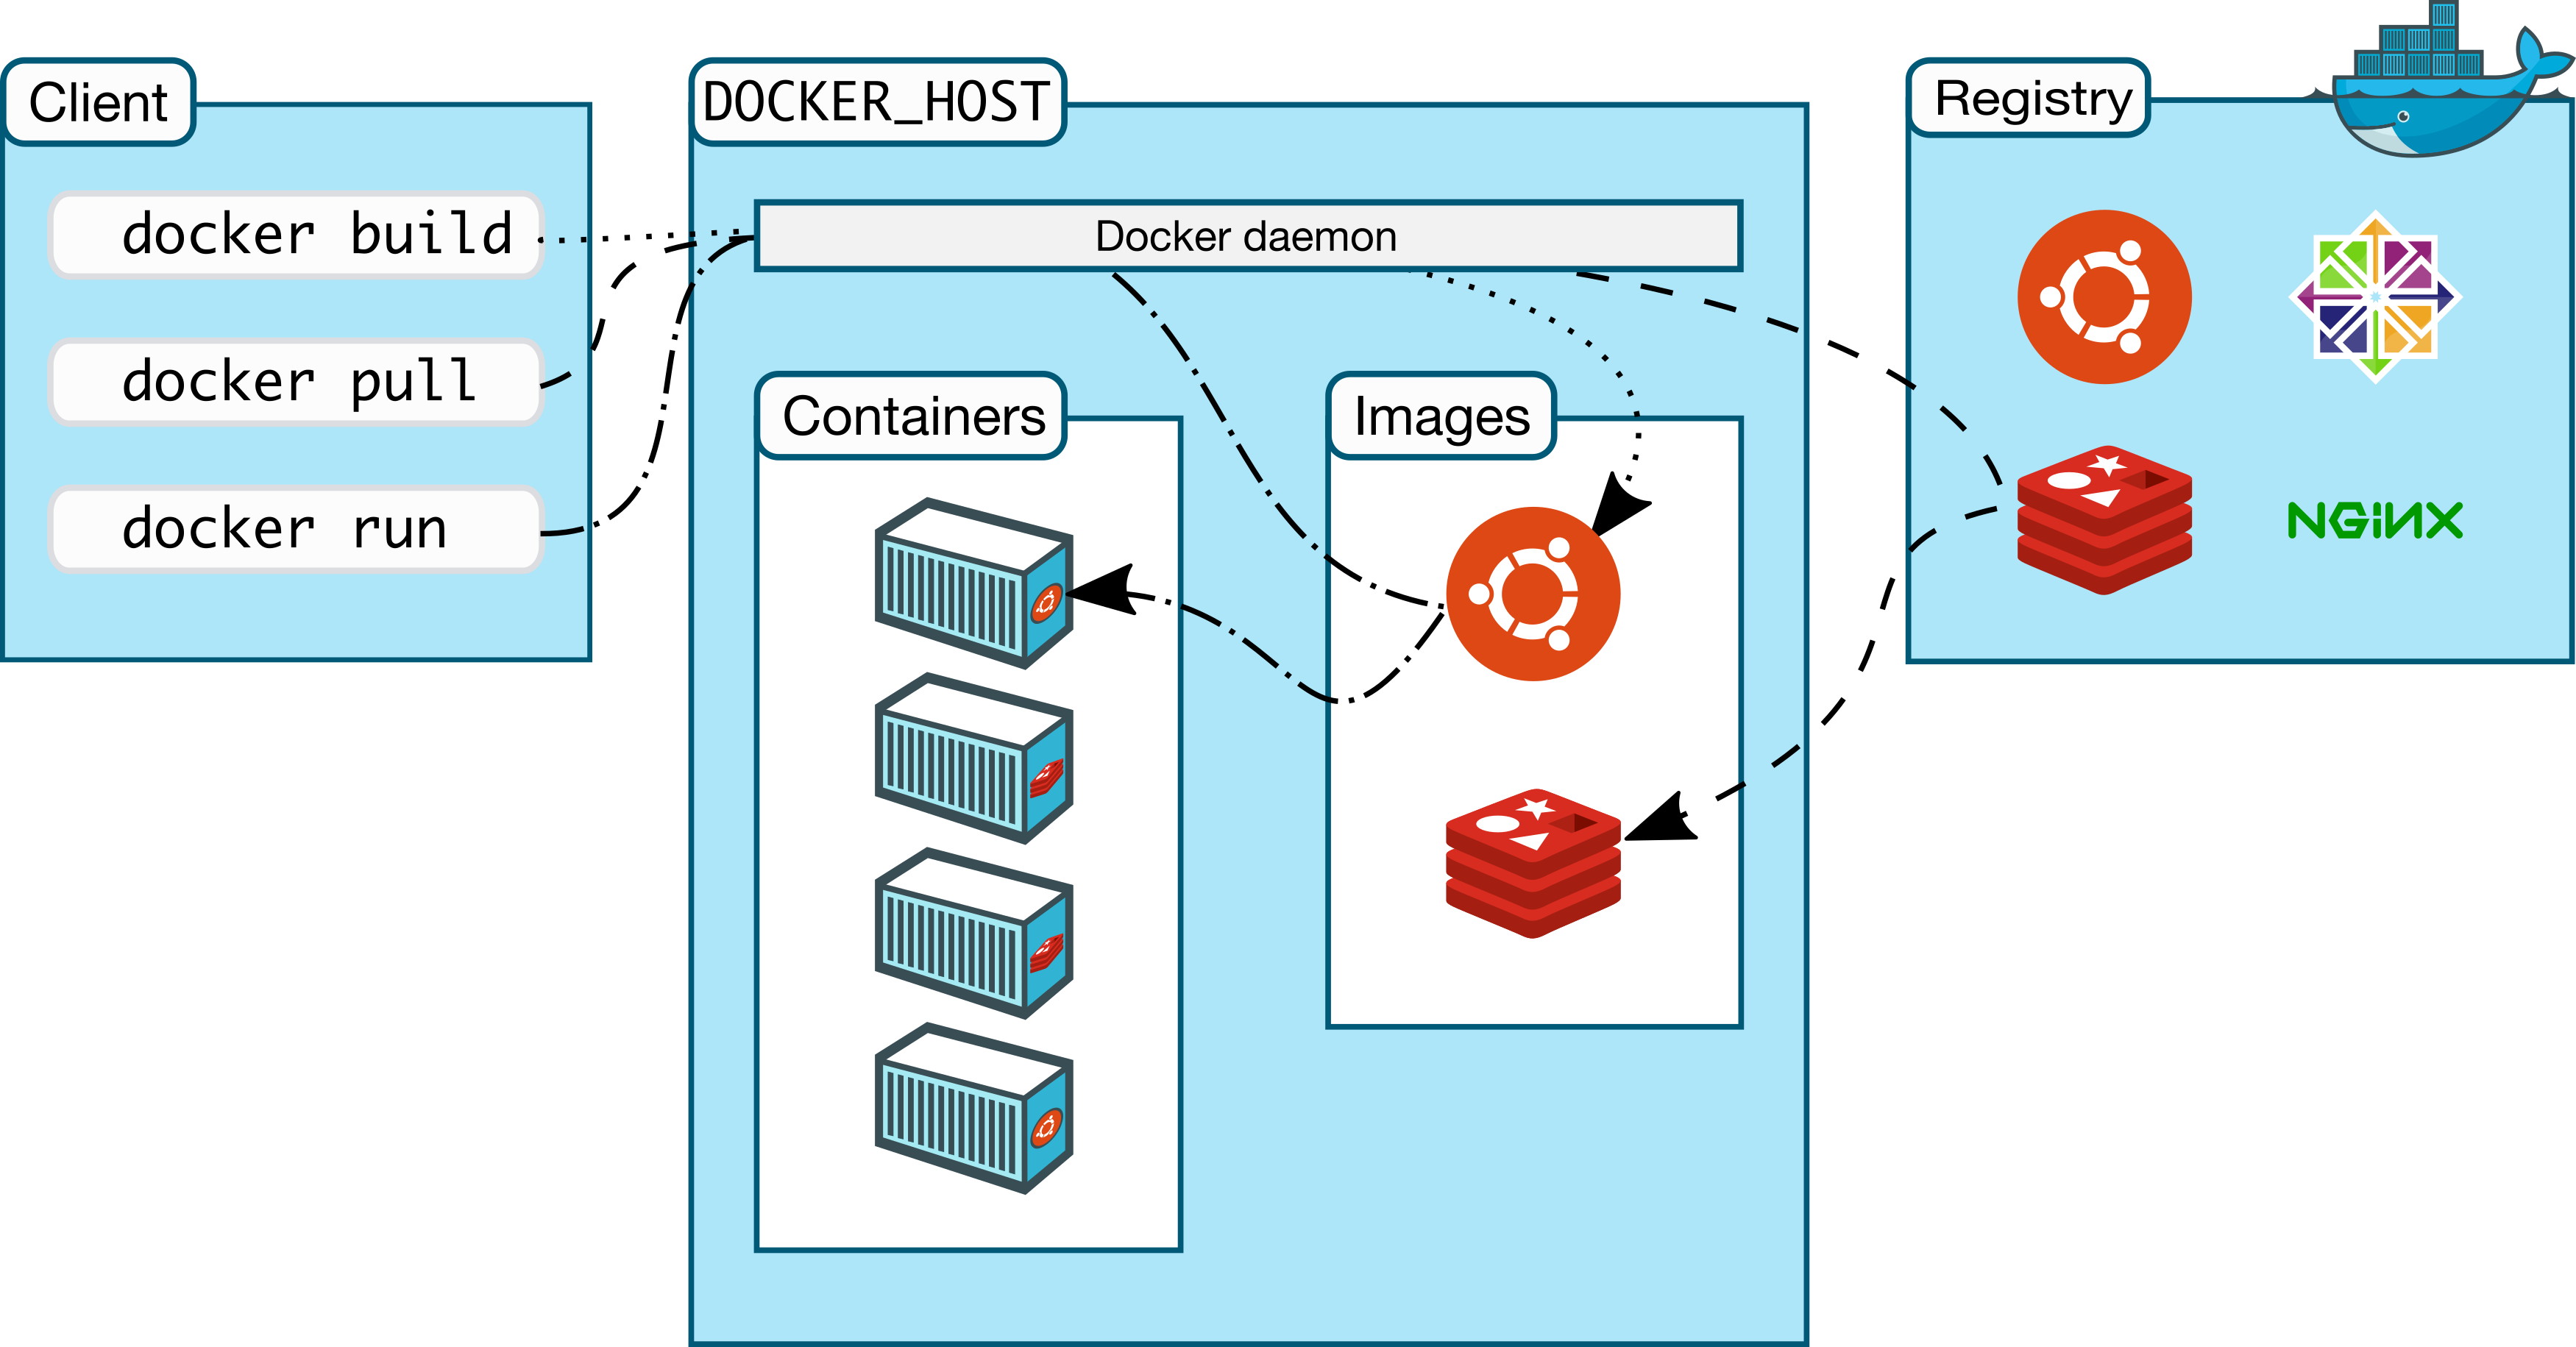
\includegraphics[width=\linewidth]{pictures/docker-arch.png}
    \caption{Arquitectura cliente--servidor de Docker \cite{DockerOverview2021}.}
    \label{fig:docker-arch}
\end{figure}

De la imagen anterior destacan tres bloques principales: el cliente, el servidor
(\textit{docker host}) y el registro (\textit{registry}). Por una parte, el cliente
es la principal forma de comunicarse con el servicio de Docker. Ejecutando comandos
como \texttt{docker run} se envían al servicio peticiones mediante la API REST interna
que gestionan los contenedores.

Por su lado, el servicio está gestionado por el \textit{Docker daemon}, llamado
\texttt{dockerd}. Dicho servicio escucha de forma activa las peticiones API entrantes
y gestiona los objetos de Docker, como las imágenes, contenedores, interfaces de red
y volúmenes. Además, un servicio puede comunicarse con otros servicios para gestionar
a su vez otros contenedores.

Finalmente, los registros de Docker (no confundir con los \textit{logs}, que también
se traduce como ``registro'') son un repositorio en donde se almacenan imágenes Docker.
Por defecto, se hace uso de Docker Hub, que es el registro principal y al cual
el servicio de Docker solicita imágenes cuando no las encuentra, y en donde cualquier
usuario puede publicar la imagen que quiera. Pero, además, una persona puede hospedar
su propio registro privado (al igual que si se desplegase un servidor Nexus).

Uno de los conceptos fundamentales que se han mencionado anteriormente son los ``objetos
Docker''. Esa nomenclatura se usa para agrupar y mencionar a todo aquello que se crea
y genera cuando se trabaja con el servicio de Docker: imágenes, contenedores, interfaces de red,
\textit{plugins}, volúmenes y demás.

\subsubsection*{Imágenes}
Una imagen conforma una plantilla de solo lectura la cual contiene instrucciones
para crear un contenedor Docker. Por lo general, las imágenes se basan en otras
ya existentes con configuraciones adicionales.

Un caso habitual es una imagen basada en \texttt{ubuntu-server} sobre la cual
se instala un servidor Apache y la aplicación NodeJS que hemos desarrollado. Con esto,
tendríamos una imagen la cual se basa en Ubuntu, que ejecuta un servidor Apache y
que tiene una aplicación NodeJS, junto con los ajustes pertinentes para un
correcto funcionamiento, definiendo así una imagen nueva (figura \ref{fig:sample-image}):

\begin{figure}[H]
    \centering
    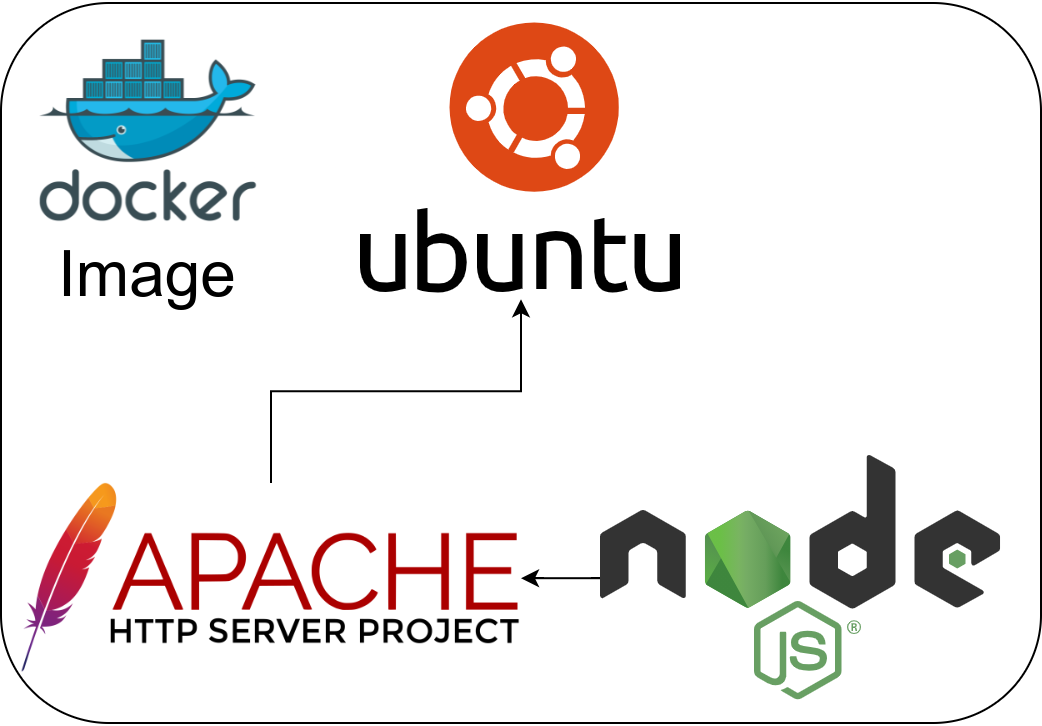
\includegraphics[width=\linewidth]{pictures/sample-image.png}
    \caption{La nueva imagen que habríamos definido basándose en las premisas anteriores.}
    \label{fig:sample-image}
\end{figure}

Cuando se quiere crear una nueva imagen se utiliza un fichero \texttt{Dockerfile}
el cual incluye las directivas necesarias para construir una imagen desde cero (o
basándose en una ya existente). Además, el funcionamiento de este tipo de ficheros
es muy similar a los \texttt{Makefile} en tanto que, cuando se realiza algún cambio
sobre el mismo, solo se reconstruyen en aquellas imágenes que hayan cambiado las
capas modificadas. Esto se traduce en imágenes mucho más pequeñas, ligeras y rápidas
en comparación, por ejemplo, a las máquinas virtuales.

\subsubsection*{Contenedores}
Un contenedor es una instancia de una imagen que puede ser ejecutada. Las operaciones
básicas sobre contenedores son: crear, iniciar, parar, mover o eliminar. Además, se
pueden conectar una o varias redes, volúmenes de datos o inclusive definir y crear
una nueva imagen a partir del estado actual.

Por defecto, un contenedor está bastante bien aislado del resto de contenedores en la
máquina anfitriona. Sin embargo, se puede definir y controlar cómo de aislada está
una red, un almacenamiento o los subsistemas que están por debajo.

Es fundamental tener en cuenta que un contenedor está directamente definido por la
imagen que lo crea y por las configuraciones iniciales que se le dan en el momento
de la creación. Sin embargo, todos los cambios efectuados durante su ciclo de vida
que no sean de imagen o de configuración desaparecerán una vez el contenedor se
detenga y se elimine (esto incluye todo el sistema de ficheros que hay por
debajo).

\subsubsection*{Almacenamiento}
Dada la situación anterior, es necesario buscar alguna manera de persistir la
información de los contenedores. Por defecto, los datos que se generan y gestionan
en un contenedor de Docker son directamente gestionados por el servicio de Docker
y se trabaja con ellos sobre una capa escribible asociada al contenedor \cite{ManageDataDocker2021}.
Esto se traduce en:

\begin{itemize}
    \item Los datos no son persistentes, por lo que eliminar el contenedor eliminará
          la información.
    \item La capa escribible de un contenedor está asociada a dicho contenedor, por
          lo que resulta complejo para otros procesos extraer información de ella.
    \item Además, dicha capa está directamente asociada a la máquina anfitriona en
          donde el contenedor está ejecutándose, por lo que es muy complejo mover
          los datos de un sitio a otro.
    \item Realizar escrituras sobre la capa escribible de un contenedor necesita de
          un driver que gestione el sistema de ficheros. Usando el kernel de Linux,
          este driver ofrece una sistema de ficheros \texttt{UnionFS}, configurado
          a partir de la unión de varios sistemas de ficheros \cite{UnionFS2020}. Esto
          conlleva una penalización en rendimiento en comparación con el uso de volúmenes
          de datos, que trabajan directamente sobre el sistema de ficheros del anfitrión.
\end{itemize}

Por defecto, existen dos formas de persistir los datos de un contenedor: mediante el
uso de volúmenes o mediante \textit{bind mounts}, es decir, asociar un directorio
en el host con un directorio en el contenedor.

\begin{figure}[H]
    \centering
    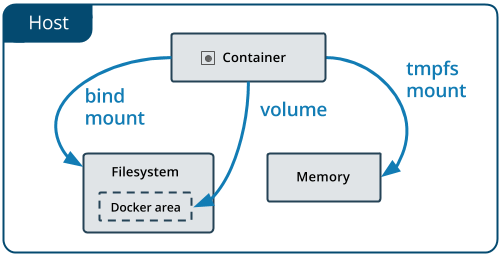
\includegraphics[width=.7\linewidth]{pictures/types-of-mounts.png}
    \caption{Posibles ubicaciones en donde se almacena la información en contenedores Docker \cite{ManageDataDocker2021}.}
\end{figure}

\subsubsection*{\indent --- Volúmenes}
Los volúmenes ofrecen un almacenamiento persistente completamente gestionado por Docker,
por lo que hay que crearlos de forma explícita con ``\lstinline[style=bash]!docker volume create!''.

Cuando se crea un volúmen, los datos se alojan directamente en la máquina anfitriona.
Si se asocia a un contenedor, el volumense monta como un directorio dentro del mismo,
mostrando un funcionamiento similar a \textit{bind mounts}. La principal diferencia
es que los volúmenes ofrecen un entorno completamente aislado de almacenamiento,
gestionado por Docker y portable.

Aprovechando lo anterior, es posible montar un volumen en varios contenedores
abriendo la posibilidad de que compartan datos entre ellos. Además,
los volúmenes son independientes de los contenedores que los usan: si ningún contenedor
usa un volúmen, este sigue existiendo hasta que se elimine manualmente (``\lstinline[style=bash]!docker volume prune!'').

Por otra parte, como los volúmenes son gestionados por Docker permite disponer de
\textit{volume drivers} para almacenar datos en equipos remotos.

Para resumir, se indican las características principales de los volúmenes \cite{UseVolumes2021}:

\begin{itemize}
    \item Son fáciles de manejar, hacer copias de seguridad y de migrar a otros servidores.
    \item Se pueden gestionar completamente desde la interfaz de línea de comandos de Docker.
    \item Funcionan tanto en Windows como en Linux.
    \item Están diseñados para que puedan ser compartidos por varios contenedores de forma segura.
    \item Se pueden almacenar los datos en equipos remotos o proveedores de servicios en la nube.
    \item El rendimiento en plataformas paganas (MacOS y Windows) es mejor que con \textit{bind mounts}.
    \item No incrementan el tamaño del contenedor sino del volumen en sí.
\end{itemize}

Los volúmenes se almacenan en el área de Docker, aislados del sistema dentro del sistema
(figura \ref{fig:volumes-location}):

\begin{figure}[H]
    \centering
    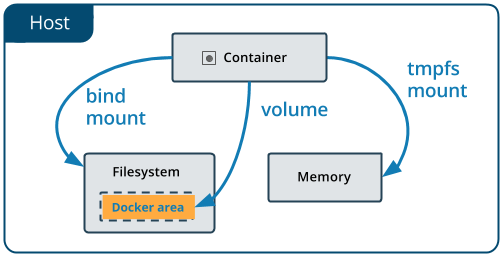
\includegraphics[width=.7\linewidth]{pictures/types-of-mounts-volume.png}
    \caption{Ubicación del almacenamiento de los volúmenes en Docker \cite{UseVolumes2021}.}
    \label{fig:volumes-location}
\end{figure}

\subsubsection*{\indent --- \textit{Bind mounts}}
Los montajes de sistema de ficheros dentro de los contenedores llevan existiendo desde
el lanzamiento inicial de Docker. Su funcionamiento es simple: utilizando los
mecanismos de los sistemas operativos anfitriones, un directorio (o fichero)
en el equipo anfitrión se monta dentro del contenedor en una ruta en específico.
Si el fichero o directorio no existe, se crea bajo demanda en el momento de la
creación del contenedor.

Es importante tener en cuenta que este tipo de sistema de ficheros está mucho más
limitado que un volumen y pueden suponer un gran fallo de seguridad en tanto a que
es posible acceder a ficheros sensibles del sistema.

Hay que tener en cuenta que los contenedores Docker siempre se ejecutan como
súper usuario (administrador), por lo que un proceso malicioso podría editar,
modificar, leer y eliminar ficheros fundamentales del sistema anfitrión si no
se ha tenido cuidado con el directorio a montar.

Sin embargo, es una opción muy interesante para almacenar datos que son modificados
con cierta regularidad o que no interesa ``persistirlos''. Por ejemplo, ficheros
de configuración (para cambiarla bajo demanda), directorios que contengan \textit{logs},
etc.

Los \textit{bind mounts} se almacenan en el sistema de ficheros anfitrión (figura \ref{fig:bind-location}):

\begin{figure}[H]
    \centering
    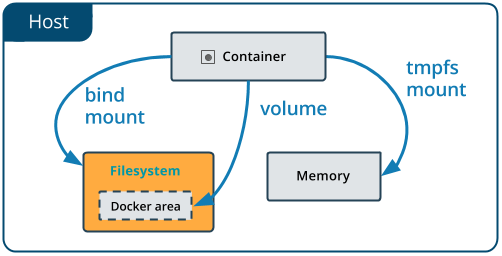
\includegraphics[width=.7\linewidth]{pictures/types-of-mounts-bind.png}
    \caption{Ubicación del almacenamiento de los \textit{bind mounts} en Docker \cite{UseBindMounts2021}.}
    \label{fig:bind-location}
\end{figure}

\subsubsection*{\indent --- ¿Cuándo usar volúmenes o \textit{bind mounts}?}
Basándose en la documentación oficial de Docker \cite{ManageDataDocker2021}, hay
unos casos para unos o para otros, según se requiera (tabla \ref{tab:mount-cases}):

\newpage

\begin{landscape}
    \begin{table}[H]
        \centering
        \begin{tabularx}{\linewidth}{C{.25}||C{.25}|C{.25}|C{.25}|C{.25}|C{.25}|C{.25}|C{.25}}
                                          & \textbf{Compartir datos entre contenedores} & \textbf{Gestionar ajustes} & \textbf{Estructura del FS} & \textbf{Copias de seguridad} & \textbf{Datos en la nube}                                     & \textbf{Alto rendimiento}                              & \textbf{Versiones del código fuente} \\
            \hline
            \textbf{Volúmenes}            & \cmark                                      & \xmark                     & \cmark                     & \cmark                       & \cmark (nativo)                                               & \cmark (en Docker Desktop)                             & \xmark                               \\
            \hline
            \textbf{\textit{Bind mounts}} & \xmark                                      & \cmark                     & \xmark                     & \xmark                       & \cmark (usando un sistema de ficheros en la nube, como SAMBA) & \cmark (depende del sistema de ficheros del anfitrión) & \cmark                               \\
            \hline
        \end{tabularx}
        \caption{Cuándo usar un tipo de almacenamiento persistente u otro, de elaboración propia basándose en la documentación \cite{ManageDataDocker2021}.}
        \label{tab:mount-cases}
    \end{table}
\end{landscape}

\subsubsection*{Interfaces de red}
Docker ofrece un potente mecanismo de gestión de redes para permitir la comunicación
entre contenedores y con elementos externos. Una de las motivaciones principales
detrás de la gestión propia de la red por parte de Docker es la de que las aplicaciones
no sepan si están dentro de un contenedor o si tienen que comunicarse con el exterior
o con una carga de trabajo externa a Docker, sino que van a comunicarse directamente
sin necesidad de ninguna configuración externa.

Indiferentemente de si el servicio se está ejecutando en una máquina Linux y otro en
una máquina Windows, la comunicación entre ellas se va a realizar completamente
independiente a la plataforma.

La gestión de las redes y aislamiento de las mismas se realiza mediante una
manipulación directa de \texttt{iptables}. Esto se hace así porque el \textit{firewall}
nativo de Linux tiene una grandísima potencia, es muy configurable y se ejecuta
directamente a nivel de kernel, lo cual reduce el \textit{overhead} que pudiera
presentar si fuese una aplicación a nivel de usuario.

Esto conlleva que las rutas del \textit{firewall} que se hubiesen creado previamente
deben aparecer antes de las creadas por Docker (para que tengan mayor peso) y 
permiten llevar la ejecución de contenedores Docker a distintos tipos de \textit{hardware}:
servidores, routers (en donde Docker actúa como router) y equipos embebidos.

Por defecto, Docker expone los siguientes drivers \cite{NetworkingOverview2021}:

\begin{itemize}
    \item \texttt{bridge}: el driver que se usa por defecto, si no se especifica 
          ninguno. Se destina este tipo de driver cuando las aplicaciones se
          ejecutan de forma aislada y solo necesitan comunicarse con el exterior o,
          si por el contrario, hace falta que múltiples contenedores se comuniquen
          entre sí.

    \item \texttt{host}: elimina el aislamiento de red con el sistema anfitrión,
          usando la interfaz del sistema (por lo que se debe ajustar
          el \textit{firewall} y la red, si necesita alguna característica especial).
        
    \item \texttt{overlay}: interconecta múltiples servicios de Docker (que pueden
          estar en máquinas distintas) para facilitar la comunicación entre clústers
          de Docker Swarm o contenedores entre sí.

    \item \texttt{macvlan}: asigna una dirección MAC al contenedor de forma que parezca
          que es una máquina física, por lo que se realiza el enrutamiento según las
          direcciones MAC.

    \item \texttt{none}: deshabilita todas las comunicaciones de red para el
          contenedor, se suele usar conjunto a un driver personalizado.

    \item \textit{Network plugins}: cada persona puede desarrollar su propio
          driver de red para que cumpla con una función específica.
\end{itemize}

\subsubsection*{Interfaz a bajo nivel}
Docker, para funcionar, necesita del kernel de Linux por debajo. ¿Por qué esta
caracterización? Todo se debe a medidas de seguridad.

Por lo general, un contenedor de Docker se asemeja mucho a los contenedores LXC 
de Linux nativos, incluyendo entre otros características de seguridad. Si observamos
los requisitos de la interfaz Docker (figura \ref{fig:docker-interface}) vemos que
inclusive hace uso de la librería de LXC:

\begin{figure}[H]
    \centering
    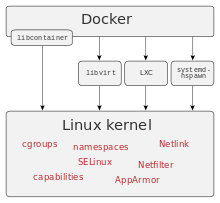
\includegraphics[width=.3\linewidth]{pictures/Docker-linux-interfaces.png}
    \caption{Interfaz de Docker con respecto al kernel de Linux. Fuente: Wikipedia \cite{DockerSoftware2021}.}
    \label{fig:docker-interface}
\end{figure}

El principal mecanismo de aislamiento son los \textit{Linux kernel namespaces},
consistentes en una ``venda en los ojos'' hacia los procesos que se ejecutan
dentro de un contenedor.

Lo siguiente que entra en juego son los \textit{control groups} (\texttt{cgroups}),
necesarios para limitar el acceso a los recursos del sistema.

Todas estas capas se analizarán en mayor profundidad más adelante, en el punto
\ref{sec:security}.
